\documentclass[a4paper,10pt]{article}

\pagestyle{empty}


%%%%%%%%%%%%%%%%%%%%%%%%%%%%%%% Paquetes %%%%%%%%%%%%%%%%%%%%%%%%%%%%%%%%%%%

\usepackage[ansinew]{inputenc}
\usepackage[spanish]{babel}
\usepackage[mathcal]{euscript}
\usepackage{amsmath,amsfonts,amssymb,theorem,latexsym,mathrsfs, %hyperref,
            epsfig, multicol,anysize,graphicx,enumitem,mdwlist}
\usepackage{graphicx}  
\usepackage{ragged2e}  
\usepackage{float}        


%%%%%%%%%%%%%%%%%%%%%%%%%%%%%%%%%%%%%%%%%%%%%%%%%%%%%%%%%%%%%%%%%%%%%%%%%%%%


%%%%%%%%%%%%%%%%%%%%%%%%%%%%%%% M�rgenes %%%%%%%%%%%%%%%%%%%%%%%%%%%%%%%%%%%

\marginsize{2cm}{1.5cm}{1cm}{2cm}

%\marginsize{izquierdo}{derecho}{arriba}{abajo}

%%%%%%%%%%%%%%%%%%%%%%%%%%%%%%%%%%%%%%%%%%%%%%%%%%%%%%%%%%%%%%%%%%%%%%%%%%%%


%%%%%%%%%%%%%%%%%%%%%%%%%%%%% Definiciones %%%%%%%%%%%%%%%%%%%%%%%%%%%%%%%%%

\def\r{\mathbb{R}}
\def\n{\mathbb{N}}
\def\q{\mathbb{Q}}
\def\c{\mathbb{C}}
\def\z{\mathbb{Z}}

\def\sen{\mathop{\mbox{\normalfont sen}}\nolimits}
\def\intt{\mathop{\mbox{\normalfont int}}\nolimits}
\def\diag{\mathop{\mbox{\normalfont diag}}\nolimits}
\def\arcsen{\mathop{\mbox{\normalfont arcsen}}\nolimits}
\def\ln{\mathop{\mbox{\normalfont ln}}\nolimits}
\def\tr{\mathop{\mbox{\normalfont tr}}\nolimits}

%%%%%%%%%%%%%%%%%%%%%%%%%%%%%%%%%%%%%%%%%%%%%%%%%%%%%%%%%%%%%%%%%%%%%%%%%%%%

\begin{document}

%%%%%%%%%%%%%%%%%%%%%%%%%%%% Encabezado %%%%%%%%%%%%%%%%%%%%%%%%%%%%%%%%%%%%

\begin{minipage}{0.12\linewidth}

\includegraphics[width=15mm]{escudo.jpg}
\end{minipage}
\begin{minipage}{0.78\linewidth}
\centerline{UNIVERSIDAD DE ANTIOQUIA}
\centerline{Facultad de Ciencias Exactas y Naturales}
\centerline{Instituto de Matem�ticas}
\centerline{Series de Tiempo II}
\centerline{Taller $\#$ 1}
\end{minipage}

\vspace{3mm}

\leftline{Profesor: Duv�n Cata�o}


\vspace{8mm}


\begin{enumerate}

\item	 For a moving average process of the form 
$$x_t = w_{t-1} + 2w_t + w_{t+1},$$
where $w_t$ are independent with zero means and variance $\sigma_w^2$, determine the autocovariance and autocorrelation functions as a function of lag $h=s-t$ and plot the ACF as a function of $h.$ 

\bigskip

\item For an $MA(1)$, $x_t = w_t + \theta w_{t-1}$, show that $|\rho_x(1)|\leq1/2$.
 for any number $\theta$. For which values of $\theta$ does $\rho_x(1)$ attain its maximum and minimum?


\bigskip

\item A real-valued function $g(t),$ defined on the integers, is non-negative definite if and only if 

$$\sum_{i=1}^{n}\sum_{j=1}^{n}a_ig(t_i-t_j)a_j\geqslant0,$$

for all positive integers $n$ and for all vectors $a=(a_1, a_2, \ldots , a_n)'$ and $t=(t_1,t_2, \ldots ,t_n)'.$ For the matrix $G=\{g(t_i-t_j); i,j = 1,2, \ldots ,n\},$ this implies that $a'Ga\geqslant0$ for all vectors $a.$ 
  \begin{enumerate}
    \item[a.] Prove that $\gamma(h),$ the autocovariance function of a stationary process, is a non-negative definite function.\\
    
     \item[b.] Verify that the sample autocovariance $\hat{\gamma}(h),$ is a non-negative definite function.\\
\end{enumerate}




 \item Consider a contrived set of data generated by tossing a fair coin, letting $x_t=1$ when a head obtained and $x_t=0$ when a tail obtained. Construt $y_t$ as $$y_t=5+x_t-0.65x_{t-1}.$$
\begin{enumerate}
\item[a.] Compare the sample ACF you obtain to the actual ACF, $\rho(h),$ with $n=10, 100, 200, 500$ and $1000.$\\

\item[b.] For each $n=10, 100, 200, 500$ and $1000,$ simulate $1000$ replications, and compute the sample ACF to lag 10, verify the Large Sample Distribution of the ACF.\\
\end{enumerate}


\item Identify the following models as ARMA$(p, q)$ models (watch out for parameter redundancy), and determine whether they are causal and/or invertible:
\begin{enumerate}
\item[a.] $x_t = 0.80x_{t-1} - 0.15x_{t-2} + w_t - 0.30w_{t-1}.$ 
\item[b.] $x_t =x_{t-1}-0.50x_{t-2}+w_t -w_{t-1}.$
\end{enumerate}
\bigskip
\item Crude oil prices in dollars per barrel are in oil; see Appendix R for more details. Fit an ARIMA$(p, d, q)$ model to the growth rate performing all necessary diagnostics. Comment.
\bigskip
\item  Fit an ARIMA$(p, d, q)$ model to the global temperature data gtemp performing all of the necessary diagnostics. After deciding on an appropriate model, forecast (with limits) the next 10 years. Comment.


\end{enumerate}

\end{document}


% \begin{figure}[H]
%  \centering
%  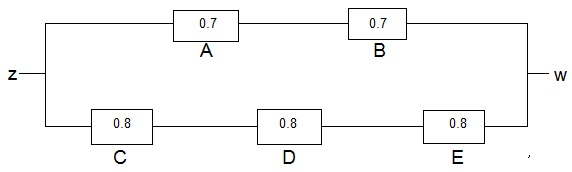
\includegraphics[width=.50\textwidth]{tab3}
% \end{figure}